\documentclass[aspectratio=169,11pt]{beamer}

\usepackage{fontspec}
\usepackage{graphicx}
\usepackage{tikz}
\usetikzlibrary{arrows.meta,positioning,calc,fit}
\usepackage{booktabs}
\usepackage{array}
\usepackage{listings}
\usepackage{xcolor}

\IfFontExistsTF{Arial}{\setsansfont{Arial}}{\setsansfont{Latin Modern Sans}}
\IfFontExistsTF{Menlo}{\setmonofont{Menlo}}{\setmonofont{Latin Modern Mono}}
\renewcommand{\familydefault}{\sfdefault}

\definecolor{bkblue}{HTML}{123B72}
\definecolor{bkcyan}{HTML}{1687A7}
\definecolor{ink}{HTML}{17212B}
\definecolor{muted}{HTML}{5C6977}
\definecolor{paper}{HTML}{F7F9FC}
\definecolor{linegray}{HTML}{D8E0E8}
\definecolor{success}{HTML}{16845B}
\definecolor{warning}{HTML}{B66A15}
\definecolor{danger}{HTML}{B63C3C}

\setbeamercolor{normal text}{fg=ink,bg=paper}
\setbeamercolor{structure}{fg=bkblue}
\setbeamercolor{frametitle}{fg=ink,bg=paper}
\setbeamercolor{title}{fg=white}
\setbeamercolor{subtitle}{fg=white}
\setbeamercolor{block title}{fg=white,bg=bkblue}
\setbeamercolor{block body}{fg=ink,bg=white}
\setbeamercolor{alerted text}{fg=danger}
\setbeamertemplate{navigation symbols}{}
\setbeamertemplate{itemize item}{\color{bkcyan}\small$\blacktriangleright$}
\setbeamertemplate{itemize subitem}{\color{bkcyan}\scriptsize$\bullet$}
\setbeamertemplate{enumerate item}{\color{bkblue}\insertenumlabel.}
\setbeamertemplate{blocks}[rounded][shadow=false]
\setbeamersize{text margin left=8mm,text margin right=8mm}

\setbeamertemplate{frametitle}{%
  \vspace{2mm}
  \begin{beamercolorbox}[wd=\paperwidth,ht=11mm,dp=2mm,leftskip=8mm,rightskip=8mm]{frametitle}
    \usebeamerfont{frametitle}\insertframetitle
    \hfill
    {\color{bkcyan}\rule{22mm}{1.2pt}}
  \end{beamercolorbox}
}

\setbeamertemplate{footline}{%
  \leavevmode
  \hbox{%
    \begin{beamercolorbox}[wd=.78\paperwidth,ht=5mm,dp=2mm,leftskip=8mm]{author in head/foot}
      \color{muted}\scriptsize CO2018 -- Simple Operating System Simulation
    \end{beamercolorbox}%
    \begin{beamercolorbox}[wd=.22\paperwidth,ht=5mm,dp=2mm,rightskip=8mm plus1fil]{date in head/foot}
      \color{muted}\scriptsize Nhóm L08 \hspace{4mm} \insertframenumber/\inserttotalframenumber
    \end{beamercolorbox}%
  }
}

\lstset{
  basicstyle=\ttfamily\small,
  keywordstyle=\color{bkcyan}\bfseries,
  commentstyle=\color{muted},
  stringstyle=\color{warning},
  backgroundcolor=\color{white},
  frame=single,
  rulecolor=\color{linegray},
  breaklines=true,
  showstringspaces=false,
  columns=fullflexible,
  aboveskip=2mm,
  belowskip=1mm
}

\newcommand{\code}[1]{\texttt{\color{bkblue}#1}}
\newcommand{\claim}[1]{\textbf{\color{bkblue}#1}}
\newcommand{\badge}[2]{%
  \tikz[baseline=(n.base)]\node[rounded corners=2pt,fill=#1!12,draw=#1!45,
  inner xsep=5pt,inner ysep=2pt,text=#1,font=\bfseries\scriptsize] (n) {#2};%
}
\newcommand{\proofchain}{%
  \begin{tikzpicture}[node distance=2.5mm,
    n/.style={draw=bkblue!40,fill=white,rounded corners=2mm,minimum height=8mm,
    inner xsep=4mm,font=\small\bfseries},
    a/.style={-{Latex[length=2mm]},thick,bkcyan}]
    \node[n] (r) {Yêu cầu};
    \node[n,right=of r] (i) {Invariant};
    \node[n,right=of i] (c) {Code};
    \node[n,right=of c] (in) {Input};
    \node[n,right=of in] (o) {Output};
    \draw[a] (r)--(i); \draw[a] (i)--(c); \draw[a] (c)--(in); \draw[a] (in)--(o);
  \end{tikzpicture}
}

\title{SIMPLE OPERATING SYSTEM SIMULATION}
\subtitle{Demo trực tiếp: từ yêu cầu đến bằng chứng tính đúng}
\author{Nhóm L08}
\date{Tháng 06/2026}

\begin{document}

% 1
\begin{frame}[plain]
  \begin{tikzpicture}[remember picture,overlay]
    \fill[bkblue] (current page.south west) rectangle (current page.north east);
    \fill[bkcyan] (current page.south west) rectangle ([xshift=9mm]current page.north west);
    \draw[white!25,line width=0.7pt] ([xshift=18mm,yshift=-15mm]current page.north west)
      rectangle ([xshift=-18mm,yshift=15mm]current page.south east);
    \node[anchor=north east] at ([xshift=-16mm,yshift=-10mm]current page.north east)
      {
\includegraphics[height=17mm]{assets/logobkheader.png}};
  \end{tikzpicture}
  \vspace{12mm}
  {\color{bkcyan}\bfseries\large BÁO CÁO BÀI TẬP LỚN HỆ ĐIỀU HÀNH -- CO2018\par}
  \vspace{7mm}
  {\color{white}\fontsize{27}{31}\selectfont\bfseries SIMPLE OPERATING SYSTEM\\SIMULATION\par}
  \vspace{5mm}
  {\color{white!82}\Large Demo trực tiếp: từ yêu cầu đến bằng chứng tính đúng\par}
  \vfill
  \begin{columns}[T]
    \column{.55\textwidth}
      {\color{white}\small
      \textbf{Giảng viên hướng dẫn:} Thầy Hoàng Lê Hải Thanh\\
      \textbf{Lớp:} L08}
    \column{.43\textwidth}
      {\color{white}\small
      2410155 -- Trần Nhật Bảo Anh\\
      2413707 -- Nguyễn Quốc Trung\\
      2410297 -- Trần Hoàng Quốc Bảo\\
      2410046 -- Trịnh Quốc An\\
      2410841 -- Nguyễn Trường Giang}
  \end{columns}
  \vspace{2mm}
\end{frame}

% 2
\begin{frame}{Ba mệnh đề nhóm cần chứng minh}
  \begin{columns}[T,onlytextwidth]
    \column{.31\textwidth}
      \begin{block}{1. Scheduler đúng}
        \small MLQ tôn trọng priority, weighted slot và quantum; hai CPU không nhận cùng PCB.
      \end{block}
    \column{.31\textwidth}
      \begin{block}{2. Memory và syscall đúng}
        \small Region và dữ liệu được bảo toàn; kernel kiểm tra PID và frame ownership.
      \end{block}
    \column{.31\textwidth}
      \begin{block}{3. MM64 đúng}
        \small Page-table walk năm cấp, canonical validation và sparse allocation.
      \end{block}
  \end{columns}
  \vfill
  \centering
  \proofchain
  \vspace{2mm}
  \par\small\color{muted}
  Mỗi output chỉ có giá trị khi nối được với invariant và code chịu trách nhiệm.
\end{frame}

% 3
\begin{frame}{Kiến trúc: một luồng xuyên suốt từ input đến RAM}
  \centering
  \resizebox{.94\textwidth}{!}{%
  \begin{tikzpicture}[
    node distance=7mm and 5mm,
    box/.style={draw=bkblue!45,fill=white,rounded corners=2mm,minimum height=12mm,
      minimum width=27mm,align=center,font=\small\bfseries},
    kernel/.style={box,fill=bkblue!7},
    cpu/.style={box,fill=warning!10},
    a/.style={-{Latex[length=2.2mm]},thick,bkcyan}]
    \node[box] (cfg) {Configuration\\+ process code};
    \node[kernel,right=of cfg] (loader) {Loader thread\\tạo PCB};
    \node[kernel,right=of loader] (sched) {MLQ scheduler\\140 ready queues};
    \node[cpu,below right=8mm and -1mm of sched] (cpu1) {CPU thread 0};
    \node[cpu,above right=8mm and -1mm of sched] (cpun) {CPU thread \(N-1\)};
    \node[kernel,right=13mm of cpu1] (sys) {System-call\\dispatcher};
    \node[kernel,right=13mm of cpun] (mmu) {Virtual memory\\MMU};
    \node[cpu,right=13mm of sys] (ram) {MEMRAM\\MEMSWAP};
    \node[kernel,below=12mm of loader] (timer) {Timer thread\\barrier theo time slot};
    \draw[a] (cfg)--(loader); \draw[a] (loader)--(sched);
    \draw[a] (sched)--(cpu1); \draw[a] (sched)--(cpun);
    \draw[a] (cpu1)--(sys); \draw[a] (cpun)--(mmu);
    \draw[a] (sys)--(ram); \draw[a] (mmu)--(ram);
    \draw[a,dashed] (timer)--(loader); \draw[a,dashed] (timer)-|(cpu1);
    \draw[a,dashed] (timer)-|(cpun);
  \end{tikzpicture}%
  }
  \vfill
  \begin{columns}[T,onlytextwidth]
    \column{.48\textwidth}
      \small\claim{PCB là trạng thái của process:} PID, priority, PC, code, registers, kernel handle và memory context.
    \column{.48\textwidth}
      \small\claim{Vòng đời:} NEW \(\rightarrow\) READY \(\rightarrow\) RUNNING \(\rightarrow\) FINISHED; hết quantum thì quay lại READY.
  \end{columns}
\end{frame}

% 4
\begin{frame}[fragile]{Build sạch và semantic assertions tạo bằng chứng có thể lặp lại}
  \begin{columns}[T,onlytextwidth]
    \column{.54\textwidth}
      \begin{lstlisting}[language=bash,basicstyle=\ttfamily\scriptsize]
	make clean && make all
	make test
      \end{lstlisting}
      \vspace{2mm}
      \begin{itemize}
        \item \claim{Clean:} loại bỏ object/binary cũ.
        \item \claim{Build:} biên dịch và liên kết toàn bộ simulator.
        \item \claim{Execute:} chạy 23 configuration.
        \item \claim{Assert:} kiểm tra các property có ý nghĩa.
      \end{itemize}
      \vspace{2mm}
      \badge{success}{Kết quả cần thấy: All semantic output assertions passed.}
    \column{.43\textwidth}
      \centering
      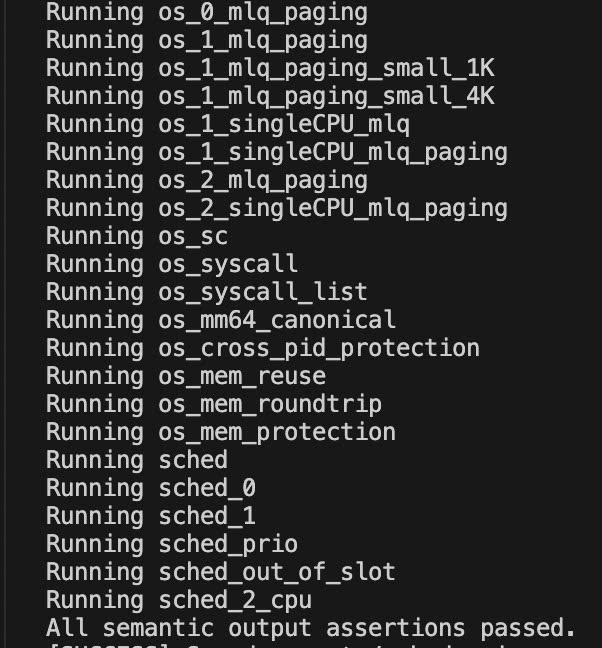
\includegraphics[height=.57\textheight]{assets/evidence_all_tests.jpg}
  \end{columns}
  \vfill
  \small\color{muted}
  Build/test pass là bằng chứng hữu hạn cho các input đã chạy, không phải chứng minh rằng chương trình không còn mọi bug.
\end{frame}

% 5
\begin{frame}{Scheduler kết hợp ba cơ chế khác nhau}
  \small
  \begin{columns}[T,onlytextwidth]
    \column{.48\textwidth}
      \begin{block}{Giữa các priority queue}
        \small Priority nhỏ hơn được quét trước; mỗi queue có quota
        \[
          slot[prio]=140-prio.
        \]
      \end{block}
      \begin{block}{Trong cùng một queue}
        \small PCB được lấy theo FIFO; process chưa xong được đưa lại cuối queue.
      \end{block}
    \column{.48\textwidth}
      \begin{block}{Mỗi lần được dispatch}
        \small Process chạy tối đa một quantum; process ưu tiên cao mới đến không preempt giữa quantum.
      \end{block}
      \begin{block}{Đa CPU}
        \small \code{queue\_lock} bảo vệ thao tác dequeue và chuyển PCB sang \code{running\_list}.
      \end{block}
  \end{columns}
  \vfill
  \centering
  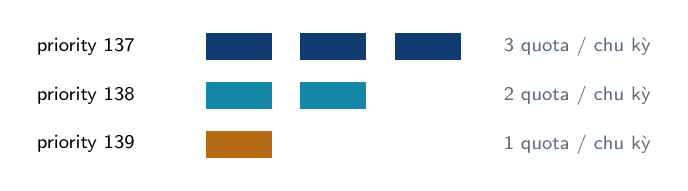
\begin{tikzpicture}[x=1.2cm,y=.62cm,font=\scriptsize]
    \foreach \p/\s/\c in {137/3/bkblue,138/2/bkcyan,139/1/warning}{
      \node[anchor=east] at (0,-\p+137) {priority \p};
      \foreach \x in {1,...,\s}
        \fill[\c] (\x-.35,-\p+136.72) rectangle (\x+.35,-\p+137.28);
      \node[anchor=west,color=muted] at (3.7,-\p+137) {\s\ quota / chu kỳ};
    }
  \end{tikzpicture}
\end{frame}

% 6
\begin{frame}[fragile]{Scheduler: bằng chứng nằm ở scheduling boundary}
  \begin{columns}[T,onlytextwidth]
    \column{.49\textwidth}
      \badge{bkblue}{Priority + quantum}
      \vspace{2mm}
      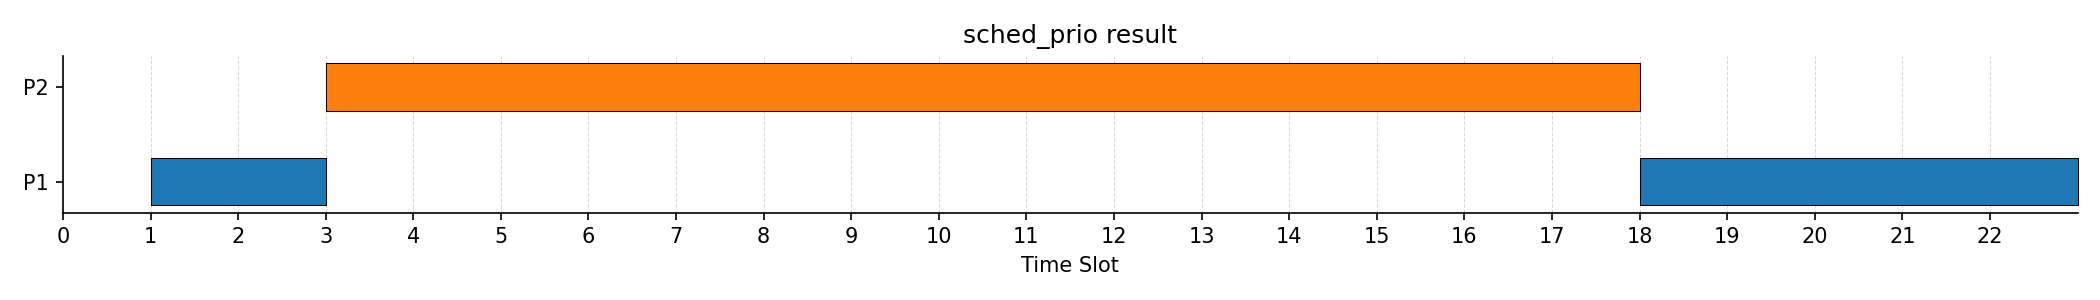
\includegraphics[width=\linewidth]{assets/sched_prio.png}
      \small
      PID priority cao đến sau chỉ được chọn khi PID hiện tại hết quantum và được put lại.
    \column{.49\textwidth}
      \badge{bkcyan}{Hai CPU, một ownership invariant}
      \vspace{2mm}
      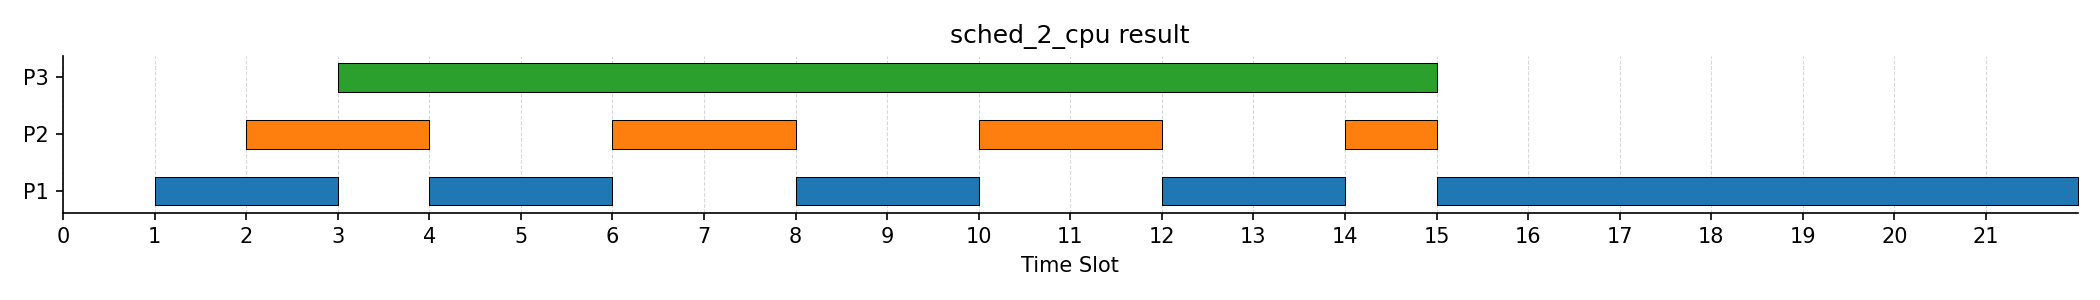
\includegraphics[width=\linewidth]{assets/sched_2_cpu.png}
      \small
      Thứ tự pthread có thể đổi; invariant là hai CPU không giữ cùng PID tại cùng thời điểm.
  \end{columns}
  \vfill
  \begin{lstlisting}[language=bash]
./os sched_2_cpu | grep -E "CPU [01]: (Dispatched|Put|Processed)"
  \end{lstlisting}
\end{frame}

% 7
\begin{frame}{Memory có ba lớp khác nhau: region, page và frame}
  \begin{columns}[T,onlytextwidth]
    \column{.52\textwidth}
      \centering
      \begin{tikzpicture}[font=\small,
        b/.style={draw=bkblue!45,fill=white,rounded corners=2mm,minimum width=45mm,
          minimum height=11mm,align=center},
        a/.style={-{Latex[length=2mm]},thick,bkcyan}]
        \node[b] (r) {\textbf{Region / VMA}\\allocation logic của process};
        \node[b,below=8mm of r] (p) {\textbf{Virtual page}\\đơn vị address translation};
        \node[b,below=8mm of p] (f) {\textbf{Physical frame}\\khối thật trong MEMRAM/MEMSWAP};
        \draw[a] (r)--node[right]{map} (p);
        \draw[a] (p)--node[right]{PTE} (f);
      \end{tikzpicture}
    \column{.45\textwidth}
      \begin{itemize}
        \item Region dùng interval half-open \([start,end)\).
        \item FREE user-region trả logical region vào free list.
        \item Page table dịch virtual page sang frame.
        \item Physical I/O đi qua syscall để kiểm tra ownership.
      \end{itemize}
  \end{columns}
  \vfill
  \claim{ALLOC path:}\quad CPU instruction \(\rightarrow\) \code{liballoc()}
  \(\rightarrow\) syscall 17 \(\rightarrow\) PID lookup \(\rightarrow\)
  \code{\_\_alloc()} \(\rightarrow\) VMA/page table/frame allocator.
\end{frame}

% 8
\begin{frame}{Region reuse: allocator tái sử dụng trước khi tăng sbrk}
  \begin{columns}[T,onlytextwidth]
    \column{.58\textwidth}
      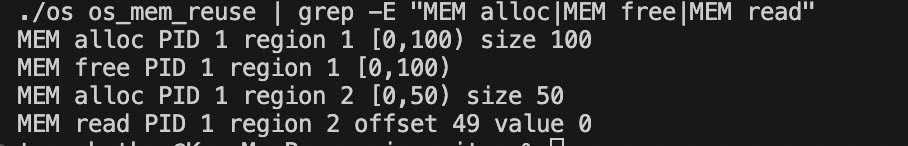
\includegraphics[width=\linewidth]{assets/evidence_mem_reuse.jpg}
      \vspace{4mm}
      \begin{tikzpicture}[x=.69mm,y=1cm,font=\small]
        \draw[thick] (0,0) rectangle (100,0.55);
        \fill[bkblue!30] (0,0) rectangle (100,.55);
        \node at (50,.275) {ALLOC region 1: \([0,100)\)};
        \draw[thick] (0,-.85) rectangle (100,-.3);
        \fill[bkcyan!35] (0,-.85) rectangle (50,-.3);
        \node at (25,-.575) {region 2: \([0,50)\)};
        \node[color=muted] at (75,-.575) {free còn lại};
      \end{tikzpicture}
    \column{.39\textwidth}
      \begin{itemize}
        \item Region 1 được free thành \([0,100)\).
        \item Allocation 50 byte nhận lại \([0,50)\).
        \item Offset 49 hợp lệ; offset 50 phải bị từ chối.
      \end{itemize}
      \vspace{3mm}
      \badge{warning}{Frame vật lý có thể chưa được trả.}
  \end{columns}
\end{frame}

% 9
\begin{frame}{Copy user--kernel--user bảo toàn dữ liệu end-to-end}
  \centering
  \begin{tikzpicture}[node distance=7mm,
    b/.style={draw=bkblue!45,fill=white,rounded corners=2mm,minimum width=35mm,
      minimum height=13mm,align=center,font=\small\bfseries},
    k/.style={b,fill=warning!10},
    a/.style={-{Latex[length=2mm]},thick,bkcyan}]
    \node[b] (u1) {User region 1\\byte \(65\)};
    \node[k,right=of u1] (k2) {Kernel region 2\\byte \(65\)};
    \node[b,right=of k2] (u3) {User region 3\\đọc lại \(65\)};
    \draw[a] (u1)--node[above,font=\scriptsize]{copy\_from\_user} (k2);
    \draw[a] (k2)--node[above,font=\scriptsize]{copy\_to\_user} (u3);
  \end{tikzpicture}
  \vspace{2mm}
  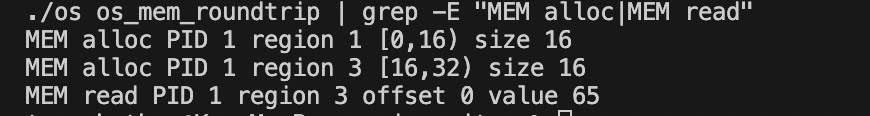
\includegraphics[width=.9\linewidth]{assets/evidence_roundtrip.jpg}
  \vfill
  \begin{columns}[T,onlytextwidth]
    \column{.56\textwidth}
      \small Cú pháp đặc tả mặc định copy một byte:
      \code{copy\_from\_user src dst}, \code{copy\_to\_user src dst offset}.
    \column{.4\textwidth}
      \small Bằng chứng nối parser, syscall, helper copy và address translation.
  \end{columns}
\end{frame}

% 10
\begin{frame}{Syscall là ranh giới kiểm soát, không chỉ là dispatcher}
  \small
  \centering
  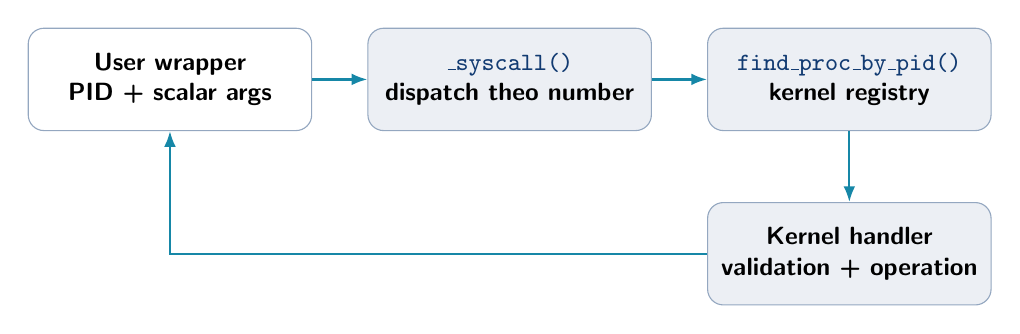
\begin{tikzpicture}[node distance=7mm,
    b/.style={draw=bkblue!45,fill=white,rounded corners=2mm,minimum width=36mm,
      minimum height=13mm,align=center,font=\small\bfseries},
    k/.style={b,fill=bkblue!8},
    a/.style={-{Latex[length=2mm]},thick,bkcyan}]
    \node[b] (user) {User wrapper\\PID + scalar args};
    \node[k,right=of user] (disp) {\code{\_syscall()}\\dispatch theo number};
    \node[k,right=of disp] (lookup) {\code{find\_proc\_by\_pid()}\\kernel registry};
    \node[k,below=9mm of lookup] (handler) {Kernel handler\\validation + operation};
    \draw[a] (user)--(disp); \draw[a] (disp)--(lookup);
    \draw[a] (lookup)--(handler); \draw[a] (handler)-|(user);
  \end{tikzpicture}
  \vspace{5mm}
  \begin{columns}[T,onlytextwidth]
    \column{.48\textwidth}
      \begin{block}{Đặc tả yêu cầu}
        \small Không truyền trực tiếp PCB pointer qua ranh giới user/kernel; kernel lookup caller bằng PID.
      \end{block}
    \column{.48\textwidth}
      \begin{block}{Unified syscall 17}
        \small Tập trung map, alloc/free/read/write, physical I/O, copy và kernel-memory operations.
      \end{block}
  \end{columns}
\end{frame}

% 11
\begin{frame}[fragile]{Biết địa chỉ vật lý không đồng nghĩa có quyền truy cập}
  \small
  \begin{columns}[T,onlytextwidth]
    \column{.62\textwidth}
      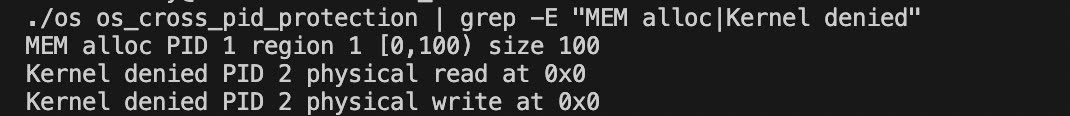
\includegraphics[width=\linewidth]{assets/evidence_cross_pid.jpg}
      \vspace{4mm}
      \begin{lstlisting}[language=bash]
./os os_cross_pid_protection |
  grep -E "MEM alloc|Kernel denied"
      \end{lstlisting}
    \column{.35\textwidth}
      \begin{itemize}
        \item PID 1 cấp region nằm trên frame 0.
        \item PID 2 biết địa chỉ 0.
        \item Kernel lookup PCB thật của PID 2.
        \item Hàm kiểm tra ownership không tìm thấy frame 0 trong page table PID 2.
      \end{itemize}
      \vspace{2mm}
      \badge{danger}{Translation \(\neq\) authorization}
  \end{columns}
\end{frame}

% 12
\begin{frame}{MM64 chia địa chỉ 57-bit thành năm cấp}
  \centering
  \begin{tikzpicture}[font=\small, x=1.45cm]
    \foreach \x/\name/\bits/\col in {
      0/PGD/56--48/bkblue,
      1/P4D/47--39/bkcyan,
      2/PUD/38--30/bkblue,
      3/PMD/29--21/bkcyan,
      4/PT/20--12/bkblue}{
      \fill[\col!18] (\x,0) rectangle (\x+1,1);
      \draw[\col!65,thick] (\x,0) rectangle (\x+1,1);
      \node[font=\bfseries] at (\x+.5,.62) {\name};
      \node[font=\scriptsize,color=muted] at (\x+.5,.28) {\bits};
    }
    \fill[warning!18] (5,0) rectangle (6.35,1);
    \draw[warning!65,thick] (5,0) rectangle (6.35,1);
    \node[font=\bfseries] at (5.675,.62) {Offset};
    \node[font=\scriptsize,color=muted] at (5.675,.28) {11--0};
    \node[anchor=west,color=muted] at (0,-.45) {Mỗi index: 9 bit = 512 entry};
    \node[anchor=east,color=muted] at (6.35,-.45) {Offset: 12 bit = page 4 KiB};
  \end{tikzpicture}
  \vspace{5mm}
  \begin{columns}[T,onlytextwidth]
    \column{.48\textwidth}
      \begin{block}{Vì sao nhiều cấp?}
        \small Flat table cần \(2^{45}\) PTE \(\times 8\) byte = \(256\) TiB cho một address space.
      \end{block}
    \column{.48\textwidth}
      \begin{block}{Canonical address}
        \small Bit 63--57 phải sign-extend bit 56; địa chỉ sai bị từ chối trước page-table walk.
      \end{block}
  \end{columns}
\end{frame}

% 13
\begin{frame}{Sparse allocation chỉ tạo bảng cho nhánh thực sự được dùng}
  \small
  \begin{columns}[T,onlytextwidth]
    \column{.48\textwidth}
      \centering
      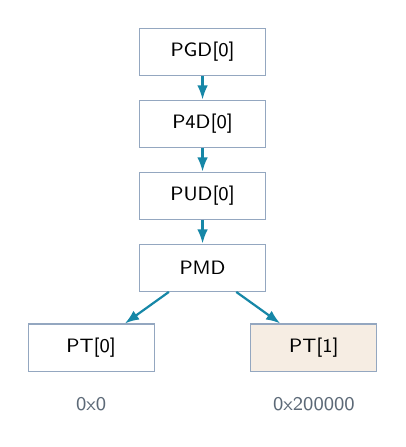
\begin{tikzpicture}[font=\scriptsize,
        n/.style={draw=bkblue!45,fill=white,minimum width=16mm,minimum height=6mm},
        a/.style={-{Latex[length=1.8mm]},thick,bkcyan}]
        \node[n] (pgd) {PGD[0]};
        \node[n,below=3mm of pgd] (p4d) {P4D[0]};
        \node[n,below=3mm of p4d] (pud) {PUD[0]};
        \node[n,below=3mm of pud] (pmd) {PMD};
        \node[n,below left=4mm and -2mm of pmd] (pt0) {PT[0]};
        \node[n,below right=4mm and -2mm of pmd,fill=warning!12] (pt1) {PT[1]};
        \draw[a] (pgd)--(p4d); \draw[a] (p4d)--(pud); \draw[a] (pud)--(pmd);
        \draw[a] (pmd)--(pt0); \draw[a] (pmd)--(pt1);
        \node[color=muted,font=\scriptsize,below=2mm of pt0] {0x0};
        \node[color=muted,font=\scriptsize,below=2mm of pt1] {0x200000};
      \end{tikzpicture}
      \vspace{2mm}
      \parbox{.9\linewidth}{\centering\scriptsize
        Mapping đầu: \(5\times4096=20480\) byte.\\
        Nhánh PMD mới: thêm \(4096\) byte.}
    \column{.49\textwidth}
      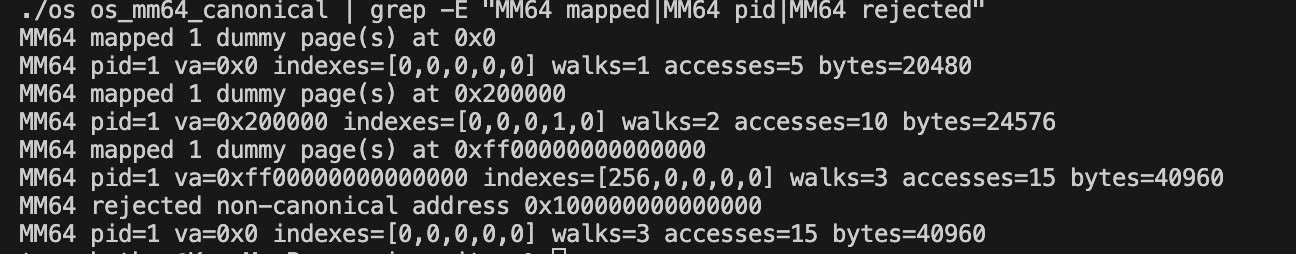
\includegraphics[width=\linewidth,height=.19\textheight,keepaspectratio]{assets/evidence_mm64.jpg}
      \vspace{2mm}
      \small
      \begin{itemize}
        \item \code{[0,0,0,0,0]}: low canonical.
        \item \code{[0,0,0,1,0]}: thêm PT branch.
        \item \code{[256,0,0,0,0]}: high canonical.
        \item Non-canonical bị từ chối.
      \end{itemize}
  \end{columns}
\end{frame}

% 14
\begin{frame}[fragile]{Semantic assertions kiểm tra property, không so toàn bộ log}
  \begin{columns}[T,onlytextwidth]
    \column{.50\textwidth}
      \begin{lstlisting}[language=bash,basicstyle=\ttfamily\scriptsize]
assert_contains output/os_cross_pid_protection.output \
  "Kernel denied PID 2 physical read at 0x0"

assert_contains output/os_mem_reuse.output \
  "MEM alloc PID 1 region 2 [0,50)"

assert_contains output/os_mm64_canonical.output \
  "MM64 rejected non-canonical address"

assert_contains output/os_mem_roundtrip_spec.output \
  "MEM read PID 1 region 3 offset 0 value 65"
      \end{lstlisting}
    \column{.46\textwidth}
      \begin{block}{Tại sao không dùng diff toàn bộ?}
        \small Pthread scheduling có thể làm các dòng độc lập đổi thứ tự dù invariant vẫn đúng.
      \end{block}
      \begin{block}{Ba tầng kiểm tra}
        \small
        \begin{enumerate}
          \item Build thành công.
          \item Execution không crash.
          \item Semantic property được assert.
        \end{enumerate}
      \end{block}
  \end{columns}
\end{frame}

% 15
\begin{frame}{Traceability: mỗi yêu cầu có code và bằng chứng cụ thể}
  \tiny
  \renewcommand{\arraystretch}{1.25}
  \begin{tabular}{>{\bfseries}p{.18\linewidth}p{.24\linewidth}p{.18\linewidth}p{.30\linewidth}}
    \toprule
    Property & Code chịu trách nhiệm & Demo & Bằng chứng quan sát\\
    \midrule
    Priority tại quantum boundary & get\_mlq\_proc(), cpu\_routine() &
      \code{sched\_prio} & PID ưu tiên cao chỉ dispatch sau khi PID hiện tại được put\\
    Không dispatch trùng PCB & queue\_lock, running\_list &
      \code{sched\_2\_cpu} & Hai CPU giữ PID khác nhau\\
    Free-region reuse & \_\_free(), get\_free\_vmrg\_area() &
      \code{os\_mem\_reuse} & Region mới nhận lại \([0,50)\)\\
    Cross-PID isolation & PID lookup, ownership check &
      cross-PID protection & PID 2 bị từ chối frame thuộc PID 1\\
    Canonical MM64 & canonical check, walk\_pte() &
      MM64 canonical & Low/high accepted; invalid rejected; bytes tăng theo branch\\
    \bottomrule
  \end{tabular}
  \vfill
  \centering
  \resizebox{.96\textwidth}{!}{\proofchain}
\end{frame}

% 16
\begin{frame}{Quyết định thiết kế và trade-off}
  \begin{columns}[T,onlytextwidth]
    \column{.48\textwidth}
      \begin{block}{Quyết định chính}
        \small
        \begin{itemize}
          \item Một \code{mm\_struct} trên mỗi process.
          \item PID lookup trong kernel.
          \item FIFO trong từng MLQ bucket.
          \item Global locks ưu tiên tính đúng.
          \item Sparse page-table tree cấp động.
        \end{itemize}
      \end{block}
    \column{.48\textwidth}
      \begin{block}{Đổi lại}
        \small
        \begin{itemize}
          \item PID lookup tuyến tính.
          \item Queue mảng làm dequeue \(O(n)\).
          \item Global memory lock giảm parallelism.
          \item Sparse walk phức tạp hơn flat table.
          \item Unified syscall có switch và argument convention lớn.
        \end{itemize}
      \end{block}
  \end{columns}
\end{frame}

% 17
\begin{frame}{Nhóm nói rõ những gì chưa được chứng minh}
  \small
  \begin{columns}[T,onlytextwidth]
    \column{.48\textwidth}
      \begin{block}{Giới hạn hiện tại}
        \small
        \begin{itemize}
          \item Page replacement chưa có test end-to-end.
          \item Chưa stress swap-full/out-of-memory.
          \item Chưa chạy ThreadSanitizer/AddressSanitizer.
          \item Chưa mô phỏng TLB và hardware interrupt thật.
          \item Free-region list chưa coalescing.
        \end{itemize}
      \end{block}
    \column{.48\textwidth}
      \begin{block}{Hướng cải tiến}
        \small
        \begin{itemize}
          \item Lock riêng theo address space.
          \item PID registry hiệu quả hơn.
          \item Stress/race/invalid-input tests.
          \item Hoàn thiện swap-out/swap-in và replacement.
          \item Thống nhất rõ granularity giữa MM64 hierarchy và data path.
        \end{itemize}
      \end{block}
  \end{columns}
  \vfill
  \centering
  \badge{warning}{Test pass chứng minh property đã assert trên input đã chạy, không chứng minh mọi execution.}
\end{frame}

% 18
\begin{frame}{Kết luận: ba nhóm invariant đã có bằng chứng lặp lại được}
  \begin{columns}[T,onlytextwidth]
    \column{.31\textwidth}
      \begin{block}{Scheduler}
        \small Priority/quantum/weighted slot và ownership PCB đa CPU.
      \end{block}
    \column{.31\textwidth}
      \begin{block}{Memory + syscall}
        \small Region/data integrity và cross-PID frame protection.
      \end{block}
    \column{.31\textwidth}
      \begin{block}{MM64}
        \small Canonical validation, five-level walk và sparse allocation.
      \end{block}
  \end{columns}
  \vspace{8mm}
  \centering
  \proofchain
  \vfill
  {\Large\bfseries\color{bkblue}Cảm ơn thầy. Nhóm sẵn sàng demo trực tiếp và trả lời phản biện.}
\end{frame}

% 19 appendix
\appendix
\begin{frame}[fragile]{Dự phòng: các lệnh demo trực tiếp}
  \begin{columns}[T,onlytextwidth]
    \column{.49\textwidth}
      \begin{lstlisting}[language=bash,basicstyle=\ttfamily\scriptsize]
# Scheduler
./os sched_prio |
  grep -E "Loaded|Dispatched|Put process|finished"
./os sched_out_of_slot |
  grep -E "Dispatched|Put process|finished"
./os sched_2_cpu |
  grep -E "CPU [01]: (Dispatched|Put|Processed)"

# Memory
./os os_mem_reuse |
  grep -E "MEM alloc|MEM free|MEM read"
      \end{lstlisting}
    \column{.49\textwidth}
      \begin{lstlisting}[language=bash,basicstyle=\ttfamily\scriptsize]
# Copy / syscall / protection
./os os_mem_roundtrip_spec |
  grep -E "MEM alloc|MEM read"
./os os_syscall_list |
  grep -E "0-sys|17-sys|440-sys"
./os os_cross_pid_protection |
  grep -E "MEM alloc|Kernel denied"

# MM64
./os os_mm64_canonical |
  grep -E "MM64 mapped|MM64 pid|MM64 rejected"
      \end{lstlisting}
  \end{columns}
\end{frame}

% 20 appendix
\begin{frame}{Dự phòng: câu trả lời nhanh khi bị hỏi sâu}
  \scriptsize
  \renewcommand{\arraystretch}{1.2}
  \begin{tabular}{>{\bfseries}p{.28\linewidth}p{.65\linewidth}}
    \toprule
    Câu hỏi & Trả lời ngắn\\
    \midrule
    Quantum khác weighted slot? & Quantum giới hạn một lần process giữ CPU; weighted slot giới hạn số lần một priority queue được chọn trong chu kỳ.\\
    Tại sao cần running list? & Registry cho PCB đang chạy; hỗ trợ PID lookup và kiểm chứng ownership ready/running.\\
    Translation khác authorization? & Translation trả lời dữ liệu ở đâu; authorization trả lời caller có quyền hay không.\\
    Vì sao năm cấp? & 45 bit virtual page number chia thành năm index 9 bit; mỗi bảng 512 entry.\\
    Vì sao test pass chưa đủ? & Chỉ chứng minh property đã assert trên input đã chạy; chưa phủ mọi race, swap-full và invalid input.\\
    Phần optional? & Page replacement hoạt động end-to-end với địa chỉ dài 64-bit phụ thuộc yêu cầu giảng viên.\\
    \bottomrule
  \end{tabular}
\end{frame}

\end{document}
